\documentclass[tikz,border=2pt]{standalone}
\usepackage{amsmath,amssymb}
\usepackage{tikz}

\begin{document}
% A x B is the set of all ordered pairs (a, b): a grid with one row per element of B and one
% column per element of A.
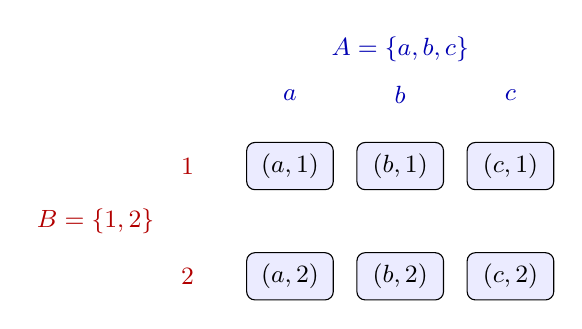
\begin{tikzpicture}[every node/.style={font=\small}]
	\foreach \x/\a in {0/a, 1.4/b, 2.8/c} {
		\node[blue!70!black, font=\small\bfseries] at (\x,2.3) {$\a$};
		\foreach \y/\b in {1.4/1, 0/2} {
			\node[draw, rounded corners=3pt, fill=blue!8, minimum width=1.1cm, minimum height=0.6cm] at (\x,\y) {$(\a,\b)$};
		}
	}
	\foreach \y/\b in {1.4/1, 0/2} {\node[red!70!black, font=\small\bfseries] at (-1.3,\y) {$\b$};}
	\node[blue!70!black, anchor=south] at (1.4,2.6) {$A=\{a,b,c\}$};
	\node[red!70!black, anchor=east] at (-1.6,0.7) {$B=\{1,2\}$};
\end{tikzpicture}
\end{document}
